\documentclass[]{article}
\usepackage{amsmath}
\usepackage{amsfonts}
\usepackage{physics}
\usepackage{graphicx}
\usepackage{fullpage}

%opening
\title{Overview of Point Group Networks}
\author{}

\begin{document}

\maketitle

$SE(3)$-Equivariant networks have proven effective in applications within the physical sciences, suggesting that physical symmetries are a useful inductive bias in the design of machine learning techniques. While $SE(3)$ networks, in principle, can fully incorporate all possible symmetries of a system, in some applications other symmetry subgroups may be more relevant. One case of this is applications of machine learning to condensed matter systems, where atoms are arranged in periodic structures where each atomic position has some point symmetry group.

In $SE(3)$ Equivariant networks, initial edge features $\vec{e}_{ij}^{L=0}$ are often spherical harmonic functions $Y_{m}^{\ell}(\vec{r}_{ab}$ evaluated for interatomic radii $\vec{r}_{ab}$ of atom pairs $(a,b)$. Point group features may be derived from interatomic radii by way of projection operators $\hat{P}_{ij}^{\mu}$, which project arbitrary vector spaces onto subspaces $V_{\mu}$ transforming as irreducible representations $\mu$ of point group $G$. While $SE(3)$ networks rely on Clebsch-Gordan expansions of tensor products of neighboring sites and filters, point group networks instead require generalized CG coefficients or `coupling coefficients' $U^{\gamma n}_{\alpha i \beta j}$ for the direct sum decompositions of point group-irreducible features:
$$
\psi_{n}^{\gamma} = \bigoplus_{\alpha i,\beta j} U^{\gamma n}_{\alpha i \beta j} \big( u^{\alpha}_i\otimes v_{j}^{\beta}\big)
$$
With these coefficients, a similar convolutional structure may be adopted, as in $SE(3)$ networks, though now instead of harmonic indices $\ell,m$ for features, we have point group irreducible representation indices $\gamma, n$:
$$
\big(v^{L+1}_{nc}\big) ^{\gamma}_{n}=\big(v^{L}_{nc}\big)^{\gamma}_n+\sum_{b\in \mathcal{N}(n)}\sum_{\alpha i, \beta j}U_{\alpha i \beta j}^{\gamma n}\big(F^{L}_c(r_{nb})\big)^{\beta }_{j}\big(v_{bc}^L \big)^{\alpha}_{i}
$$
We propose to incorporate the above techniques into a novel framework for point-group-equivariant graph networks, suited for applications where systems display particular symmetries reduced from the full rotation symmetry of $SO(3)$. One particularly relevant application is the prediction of condensed matter Hamiltonian elements. In solid-state systems based upon an underlying periodic lattice, each atomic position displays a certain point group symmetry. Thus the Hamiltonian of the system must share a simultaneous set of eigenvalues with the symmetry operations since in this case they necessarily commute. Essentially then, the Hamiltonians solutions must be indexed by the same set as the irreducible subspaces $V_{\mu}$, each of dimension $d_{\mu}$. The basis set of one-particle wavefunctions then must have a separable form:
$$
\psi^{\mu}_{nm}(\vec{r})=R_{\mu n m}(r)\Omega^{\mu}_n(\theta,\phi)
$$
where $1\leq n\leq d_{\mu}$. The radial function $R_{\mu n m}(r)$ then depends on the specific form of the Hamiltionian and may have a very complicated structure. The prediction of this functional dependence is thus a well suited for the machine learning applications discussed here. Such models provide a method by which we may predict Hamiltionian elements naturally associated with these point-group indexes, allowing for complete descriptions of interactions between neighboring sites irreducible subspaces without truncationss (such as $\ell_{max}$ in $SE(3)$ networks). 

Furthermore, these models allow for the prediction of properties that respect the known symmetries of physical systems, by reading out features that transform as the trivial representation, allowing for more intuitive predictions of scalar (totally invariant) quantities, as well as tensorial properties with desired physical symmetries.

\newpage
\section*{Example: $D_3$ System}
\begin{center}
Consider the following system, with the chosen coordinate system $(x,y,z)$ superimposed:

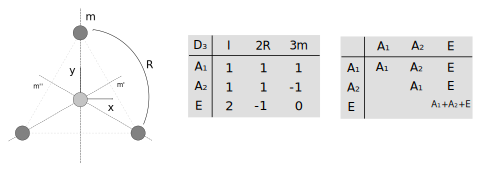
\includegraphics[scale=0.335]{d3_ex.pdf}
The rotation and mirror operations then have the following form in $\mathbb{R}^3$:
$$
I=\begin{bmatrix}
	1 & 0 &0\\
	0&1&0 \\
	0&0&1
\end{bmatrix}\quad R=\begin{bmatrix}
-\frac{1}{2} & -\frac{\sqrt{3}}{2}  &0\\
\frac{\sqrt{3}}{2}&-\frac{1}{2} &0 \\
0&0&1
\end{bmatrix}\quad R^2=\begin{bmatrix}
-\frac{1}{2} & \frac{\sqrt{3}}{2}  &0\\
-\frac{\sqrt{3}}{2}&-\frac{1}{2} &0 \\
0&0&1
\end{bmatrix}
$$
$$
m=\begin{bmatrix}
	1 & 0 &0\\
	0&-1&0 \\
	0&0&1
\end{bmatrix}\quad m'=\begin{bmatrix}
	-\frac{1}{2} & \frac{\sqrt{3}}{2}  &0\\
	\frac{\sqrt{3}}{2}&\frac{1}{2} &0 \\
	0&0&1
\end{bmatrix}\quad m''=\begin{bmatrix}
	-\frac{1}{2} & -\frac{\sqrt{3}}{2}  &0\\
	-\frac{\sqrt{3}}{2}&\frac{1}{2} &0 \\
	0&0&1
\end{bmatrix}
$$
\end{center}
In the chosen basis, the projection operators $\hat{P}^{\mu}_{i} = \frac{d_{\mu}}{N_G}\sum_{g\in G}\mathcal{D}^{\mu \dagger}(g)_{ii}\hat{O}(g)$ onto subspace basis vectors $\vert \psi^{\mu}_{i}\rangle$ of $\mathbb{R}^3$ then take the following form:
\begin{align*}
\hat{P}^{a_1}  = \begin{bmatrix}
	0 &0&0\\
	0&0&0\\
	0&0&1\\
\end{bmatrix} \quad
\hat{P}^{e}_{1}  = \begin{bmatrix}
	1 &0&0\\
	0&0&0\\
	0&0&0\\
\end{bmatrix}\quad
\hat{P}^{e}_{2} = \begin{bmatrix}
	0 &0&0\\
	0&1&0\\
	0&0&0\\
\end{bmatrix}
\end{align*}
with all other $\hat{P}^{\mu}_{i}$ vanishing over $\mathbb{R}^3$. These may be used to (here, trivially) project interatomic radii $\vec{r}_{ab}$ onto subspaces $V_{\mu}$ of $D_3$ that transform irreducibly as irreps of index $\mu$. For our three atoms $B,C,$ and $D$ neighboring $A$, we then have the following edge features:


Through convolution, these subspaces interact as tensor products of subspaces $\vert u^{\alpha}_i\rangle\otimes \vert u^{\beta}_j\rangle$ which are then reduced by way of coupling coefficients into a direct sum of another set of irreducible basis functions $\vert\psi^{\gamma}_n\rangle$.



\end{document}
